

%%-----------------------------------------------------
%%-----------------------------------------------------
\section{SSH: Trabajando desde remoto}


%-----------------------    ---------------------------------

\begin{frame}
\frametitle{¿Qué es SSH?}

\begin{itemize}
   \item Permite abrir terminales remotos
   \item La información va cifrada
   \item Máquinas de los laboratorios del GSyC
   \begin{itemize}
     \item Parte de guerra: http://sherlock.gsyc.es/parte\_de\_guerra/
   \end{itemize}
   \item \texttt{scp} permite copiar ficheros remotos
   \item Hay cliente para Windows: \texttt{PuTTY}
   \item Permite crear \emph{túneles}
\end{itemize}

\end{frame}


%-----------------------    ---------------------------------

\begin{frame}
\frametitle{SSH en acción}

\begin{center}
  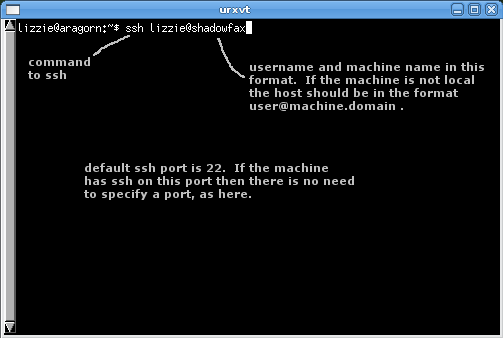
\includegraphics[width=10cm]{figs/terminal.png}
\end{center}


\begin{flushright}
{\tiny
Source: http://carina.org.uk/guidepics/terminal1.png
}
\end{flushright}

\end{frame}



%-----------------------    ---------------------------------

\begin{frame}
\frametitle{SSH}

\begin{center}
  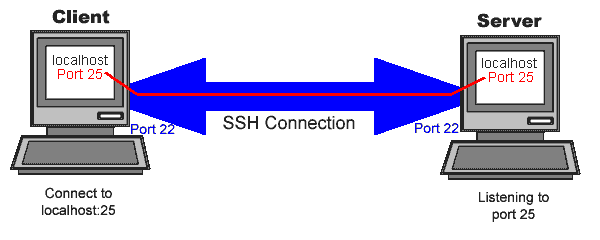
\includegraphics[width=10cm]{figs/ssh-tunnel.png}
\end{center}


\begin{flushright}
{\tiny
Source: http://www.codemastershawn.com/library/tutorial/images/ssh.tunnel.overview.gif
}
\end{flushright}

\end{frame}



